\documentclass{article}
\usepackage{tikz}
\usetikzlibrary{graphs}

\begin{document}

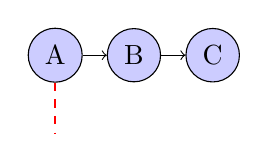
\begin{tikzpicture}

  % --- Named nodes in a graph ---
  \graph[nodes={circle, draw, fill=blue!20}, edges={->}] {
    A -> B -> C;
  };

  % --- Reuse named nodes ---
  \draw[red, thick, dashed] (A) -- ++(0,-1); % extra edge from node A

\end{tikzpicture}

\end{document}
